\documentclass[11pt]{article}

\usepackage[margin=1in]{geometry}
\usepackage{booktabs}
\usepackage{hyperref}
\usepackage{caption}
\usepackage{graphicx}
\usepackage{microtype}

\title{\bfseries Supplementary Information\\Background matching audits mass spectral antimicrobial resistance prediction}
\author{}
\date{}

\begin{document}
\maketitle

\section*{Supplementary Note 1: Why background matching is needed}

Raw external AUC answers whether a model ranks resistant isolates above susceptible isolates at a target site. It does not answer whether that ranking is driven by focal-drug biology or by the resistant population in which the label occurs. In bacterial clinical data, resistance labels are structured by lineage, mobile elements, local prescribing ecology and co-resistance. A MALDI-TOF model can exploit this structure because spectra encode abundant cellular proteins and lineage-associated peak patterns.

The background-matched audit controls the observable co-resistance component of this structure. For each focal drug, isolates are grouped by the AST labels of the other drugs in the same panel. The focal drug is excluded from the signature. Within valid strata, resistant and susceptible isolates have the same observed co-resistance background. If the model still separates them, it has residual within-background signal. If performance collapses, the original raw AUC was likely driven partly by background differences between strata.

\section*{Supplementary Note 2: Interpretation of the three AUCs}

\textbf{Raw AUC} is computed over all available isolates for the focal organism-drug-site comparison. It is the standard external performance metric.

\textbf{Matched AUC} is computed after removing strata that lack enough resistant and susceptible isolates for the focal drug. It asks whether performance remains in the subset where within-background comparisons are possible.

\textbf{Background-centered AUC} subtracts the mean model score within each valid background stratum before pooling and recomputing AUC. It is the strictest metric because it removes score shifts shared by all isolates in a background stratum.

\section*{Supplementary Note 3: How to read low-retention rows}

Low retention is not a model failure. It is an audit limitation. If a drug-site pair has few strata containing both resistant and susceptible isolates, then the data do not support a strong within-background conclusion. These rows should be reported as cautionary rather than interpreted as biological evidence.

This is why DRIAMS-B ciprofloxacin is not used as main evidence despite a high centered AUC. The estimate is based on only 25 matched isolates and one valid stratum. The method intentionally makes this visible.

\section*{Supplementary Figure 1: Background sensitivity across model families}

\begin{figure}[ht]
\centering
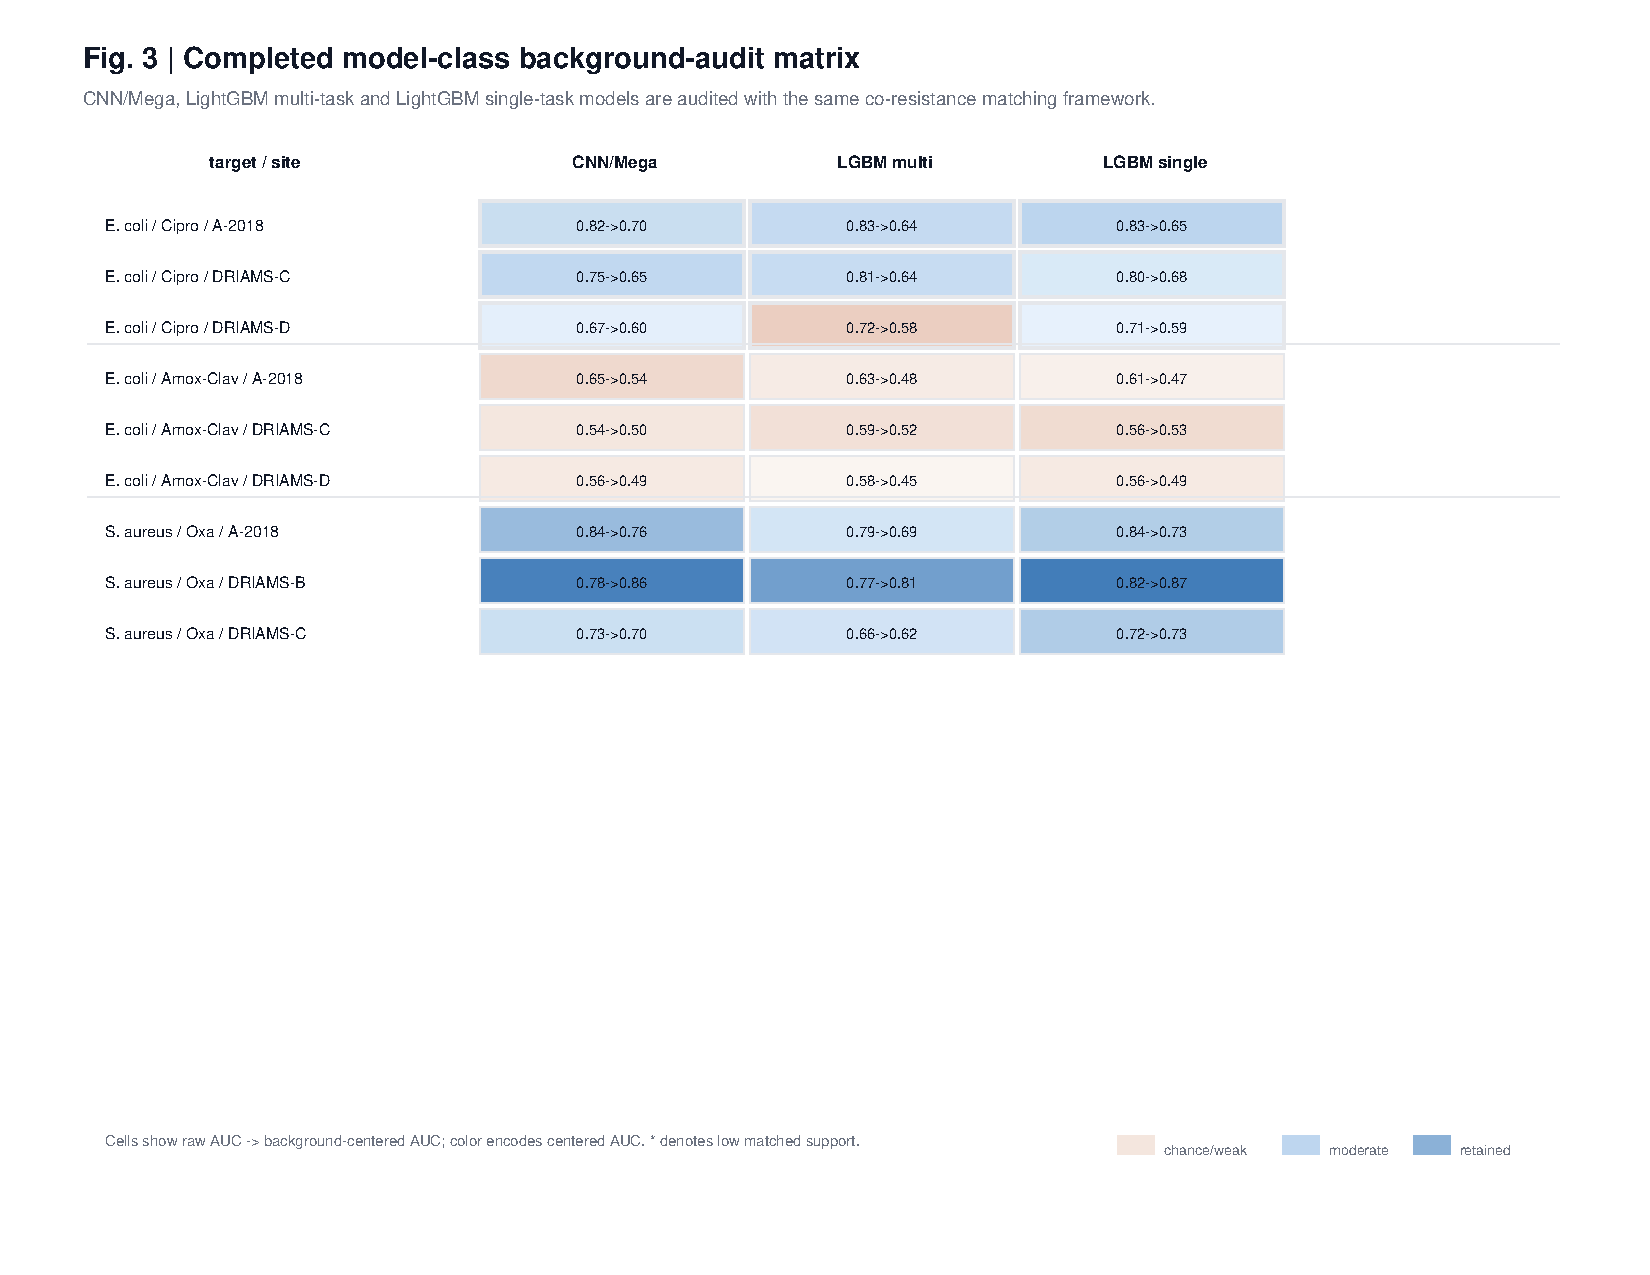
\includegraphics[width=\linewidth]{../figures/figure_3_model_family_replication.pdf}
\caption{\textbf{Background sensitivity is not specific to the convolutional model.} The same background-matched audit is applied to CNN (top) and multi-task LightGBM (bottom) predictions. Both model families show attenuation from raw to centered AUC, with stronger residual signal for ciprofloxacin than amoxicillin-clavulanic acid across the primary interpretable sites. This indicates that background sensitivity is a property of the data structure, not the architecture.}
\label{suppfig:model-replication}
\end{figure}

\section*{Supplementary Figure 2: Cross-resistance network}

\begin{figure}[ht]
\centering
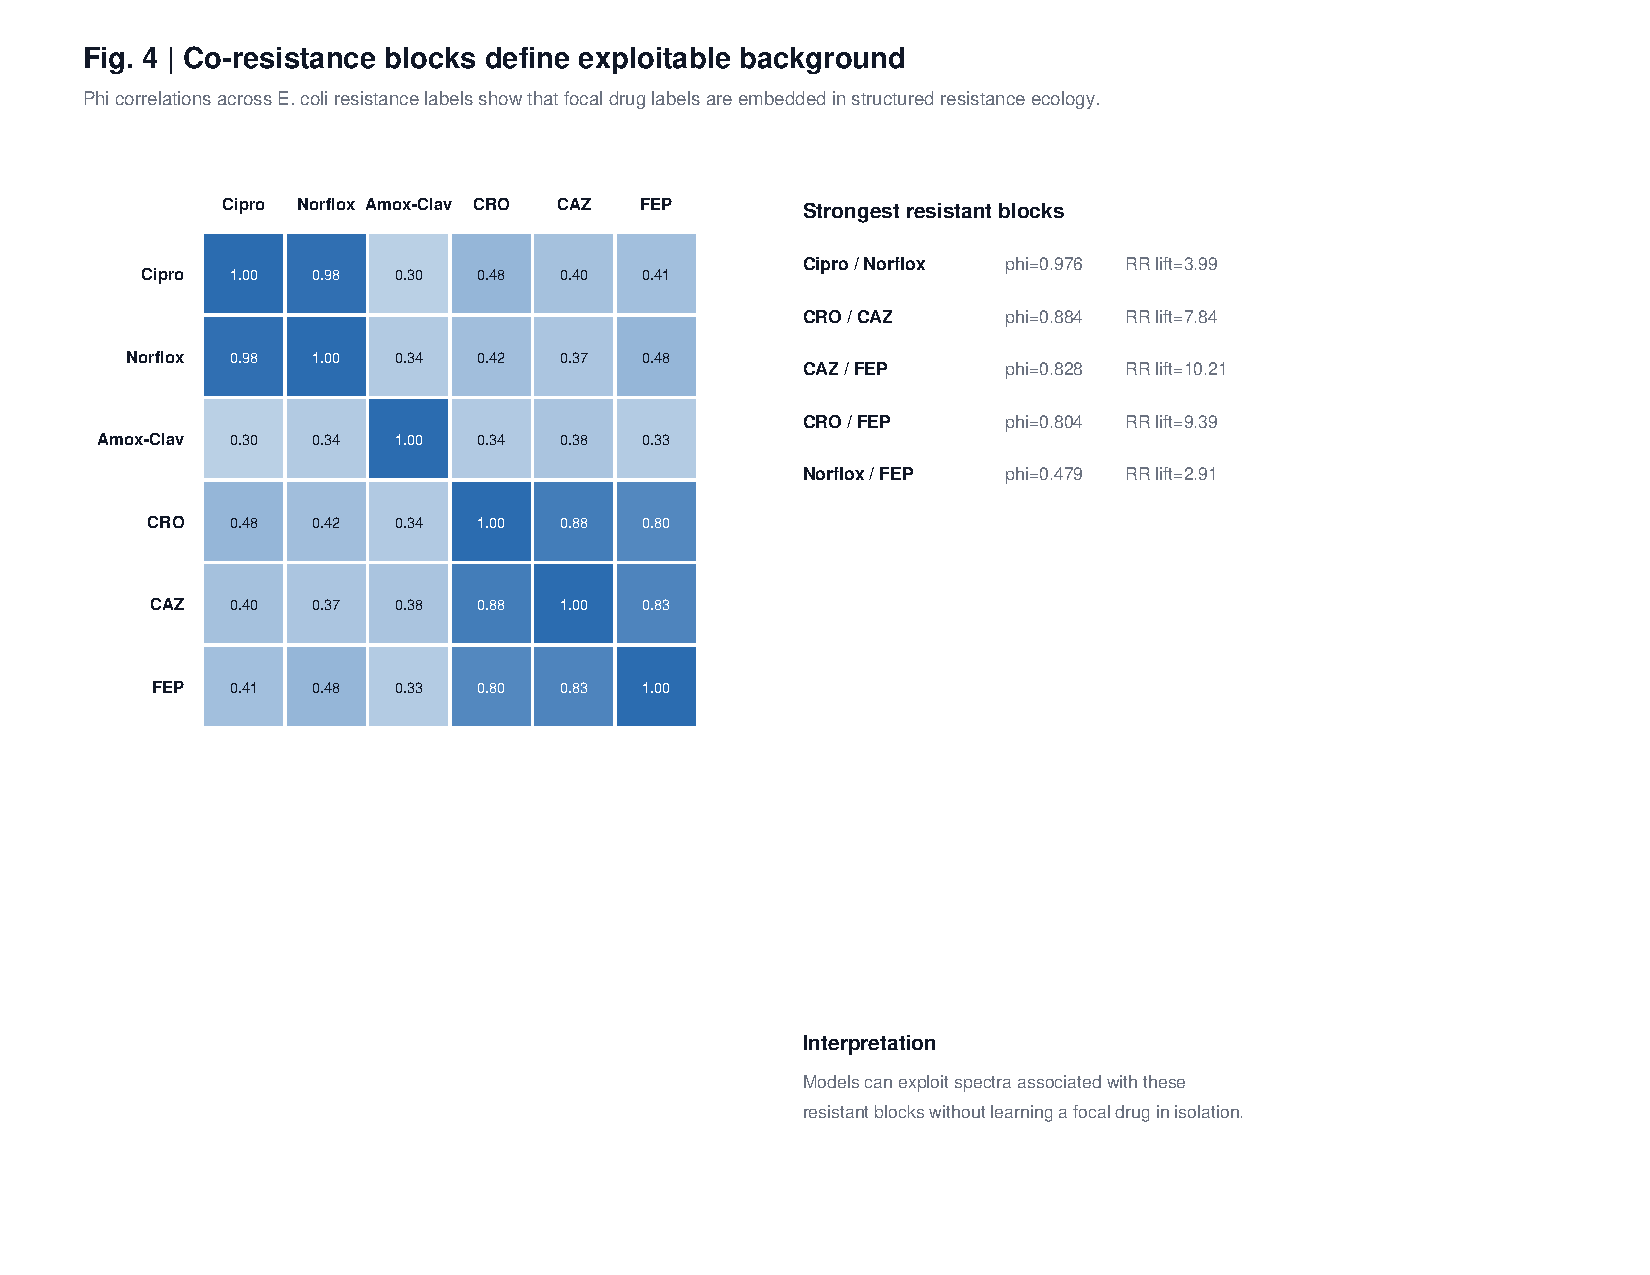
\includegraphics[width=\linewidth]{../figures/figure_4_cross_resistance_network.pdf}
\caption{\textbf{Cross-resistance network in the expanded \textit{E.~coli} panel.} Edge width and shading encode pairwise phi correlation. Two strong blocks are evident: a fluoroquinolone block (ciprofloxacin/norfloxacin, $\phi = 0.976$) and an extended-spectrum cephalosporin block (ceftriaxone, ceftazidime and cefepime, $\phi = 0.804$--$0.884$). These co-resistance structures provide exploitable background signal for any model predicting drugs within either block. Source data: \texttt{source\_data\_fig4\_cross\_resistance\_edges\_all\_sites.csv}.}
\label{suppfig:cross-resistance}
\end{figure}

\section*{Supplementary Table 1: Claim guardrails}

\begin{table}[ht]
\centering
\small
\caption{Claim guardrails used throughout the manuscript.}
\label{tab:claim-guardrails}
\resizebox{\linewidth}{!}{%
\begin{tabular}{lc}
\toprule
Status & Statement \\
\midrule
Supported & MALDI-AMR prediction is background-sensitive, and raw AUC can overstate focal-drug signal. \\
Supported & Background-centered AUC separates retained within-background ranking from background-driven attenuation. \\
Supported & Public WGS-linked Bruker data show that ST131 lineage is strongly encoded in MALDI peak features. \\
Not claimed & The DRIAMS CNN is definitively detecting ST131. \\
Not claimed & The discriminative DRIAMS or UPEC peaks have definitive protein identities. \\
Not claimed & All MALDI-AMR performance is clonal confounding. \\
\bottomrule
\end{tabular}%
}
\vspace{2mm}\parbox{0.95\linewidth}{\footnotesize These guardrails distinguish the evaluation-framework claim from direct clone or protein-identification claims.}
\end{table}


\section*{Supplementary Table 2: Source data files}

\begin{table}[ht]
\centering
\small
\caption{Source-data files distributed with the manuscript package.}
\begin{tabular}{lll}
\toprule
Display item & File & Description \\
\midrule
Figure 2 & \texttt{source\_data\_fig2\_primary\_background\_audit.csv} & Primary raw and background-centered AUC rows. \\
Figure 3 & \texttt{source\_data\_fig5a\_public\_wgs\_maldi\_auc.csv} & Public WGS-linked MALDI AUC values. \\
Figure 3 & \texttt{source\_data\_fig5b\_proteomic\_biomarker\_enrichment.csv} & ST131 biomarker enrichment values. \\
Supp.\ Fig.\ 1 & \texttt{source\_data\_fig3\_model\_family\_replication.csv} & CNN and LGBM model-family audit rows. \\
Supp.\ Fig.\ 2 & \texttt{source\_data\_fig4\_cross\_resistance\_edges\_all\_sites.csv} & Cross-resistance edges used for the phi heatmap. \\
\bottomrule
\end{tabular}
\end{table}

\section*{Supplementary Note 4: What would strengthen the biological claim}

The current evidence supports background sensitivity and the need for background-matched evaluation. It does not directly identify the DRIAMS clone or protein features. The next strongest additions would be:

\begin{itemize}
  \item WGS or MLST labels linked directly to DRIAMS isolates.
  \item Clone-controlled public WGS-linked MALDI analyses within ST131 and non-ST131 strata.
  \item Independent MALDI-AMR deployment validation on a non-DRIAMS dataset.
  \item MS/MS, MALDI-TOF/TOF or LC-MS/MS validation of discriminative m/z peaks.
\end{itemize}

\end{document}

